\section{Conceptual Model}
\label{sec:performance-modeling-conceptual-model}
A conceptual model describes the target system in terms of 
(i) the states it can assume over time, 
(ii) the events that let it change in time and
(iii) system assumptions.

We consider the conceptual model depicted in Figure~\ref{fig:conceptual-model-1} and \ref{fig:conceptual-model-2}, respectively for the system running the off-loading algorithm 1 and 2.
In both models, we introduced the \textit{Controller (CTRL)} component within the Cloudlet to represent the decision process of the off-loading policy.

\begin{figure}
	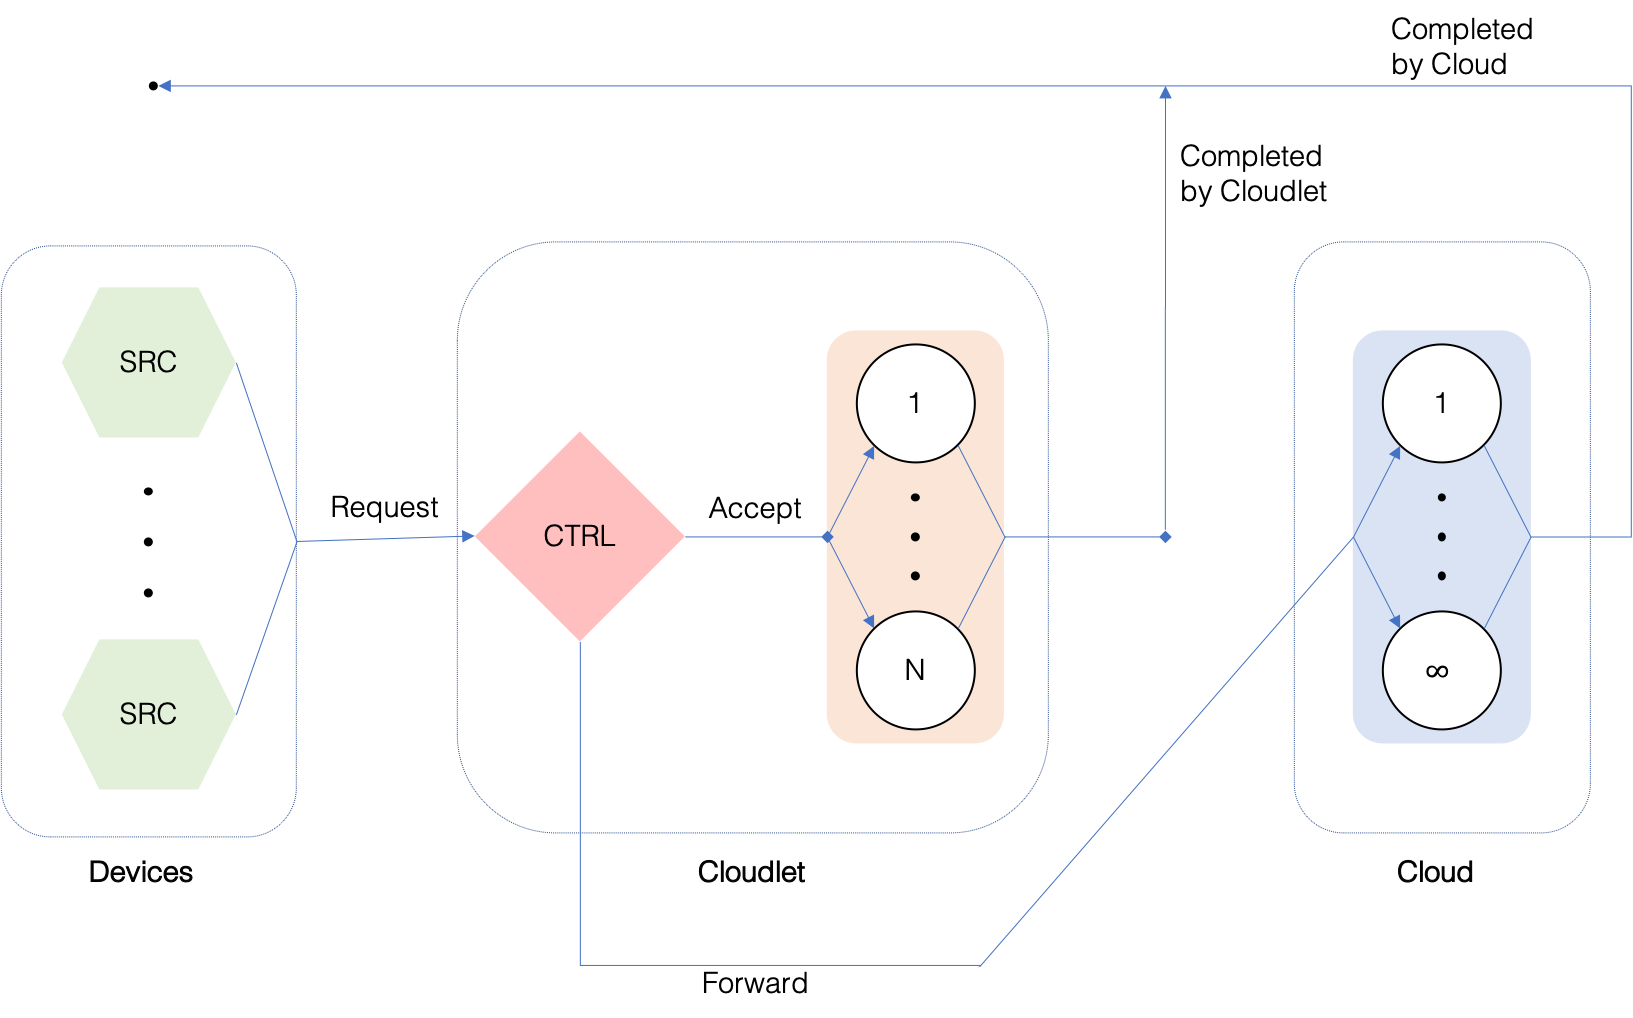
\includegraphics[width=\columnwidth]{fig/conceptual-model-1}
	\caption{Conceptual model of the system with with OP1.}
	\label{fig:conceptual-model-1}
\end{figure}

\begin{figure}
	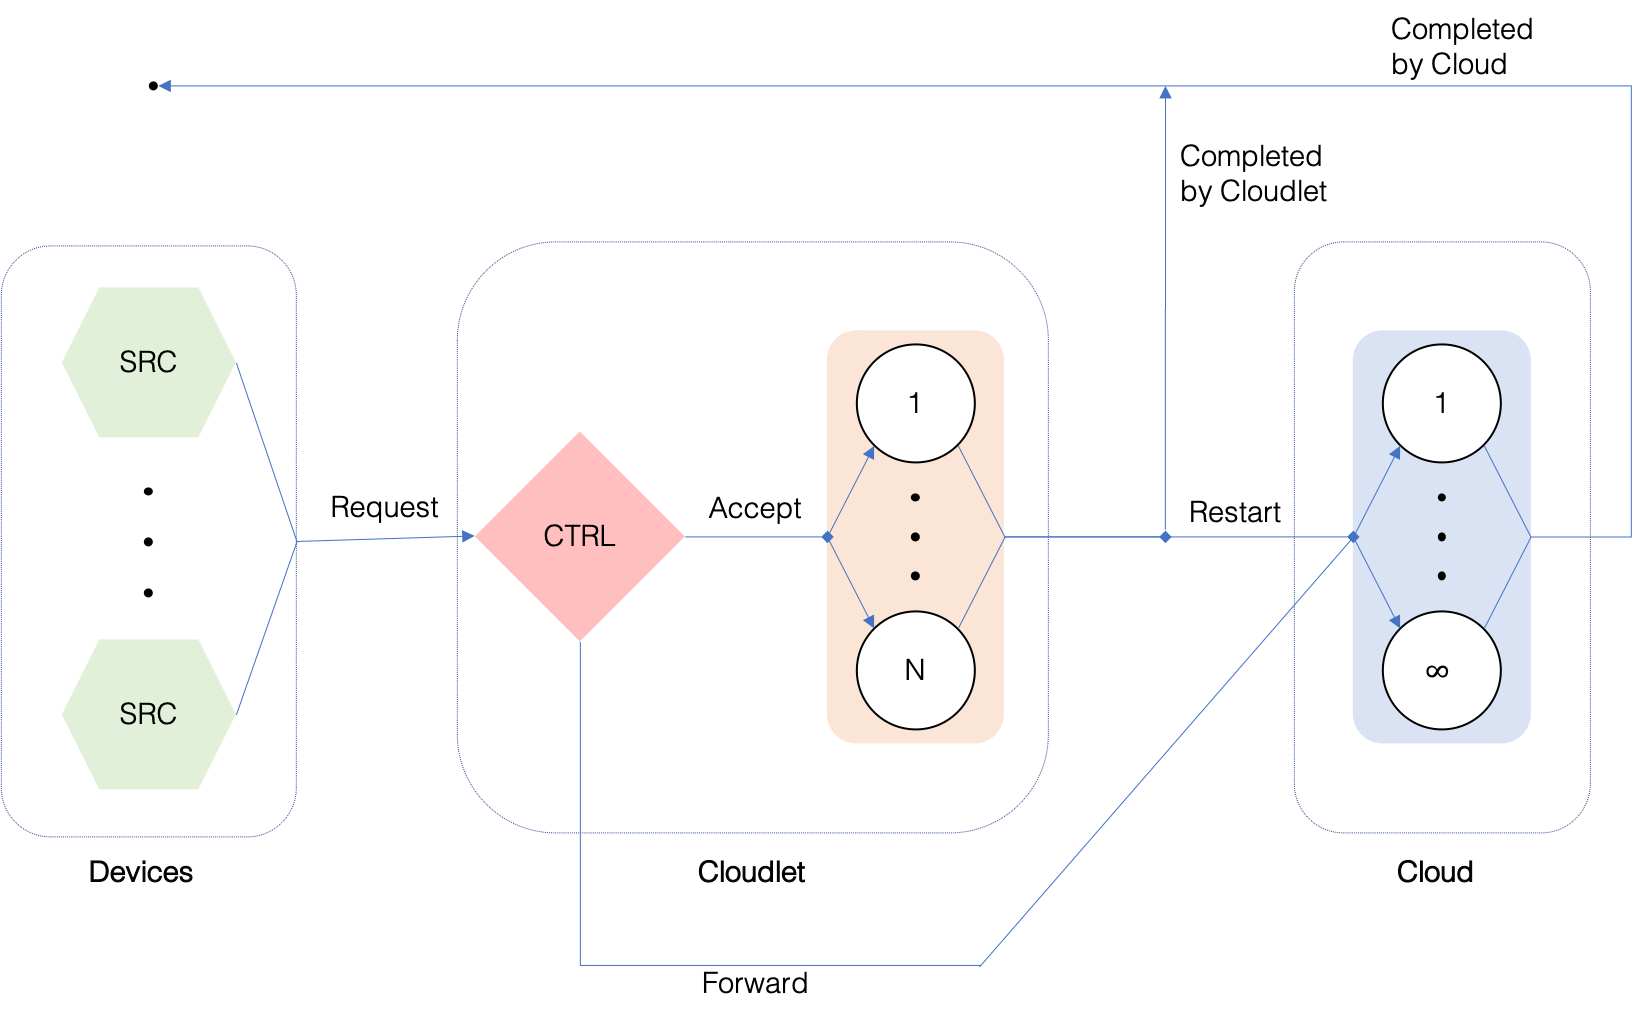
\includegraphics[width=\columnwidth]{fig/conceptual-model-2}
	\caption{Conceptual model of the system with OP2.}
	\label{fig:conceptual-model-2}
\end{figure}

\paragraph{State space}
The state space $S$ of a system is a comprehensive characterization of the system at any given time.
The state space of the whole system is represented by the state space of its subsystems:

\begin{itemize}
	\item \textbf{Cloudlet}: $S_{clt} := \{(n_{clt,1},n_{clt,2})\in \mathcal{N}^{2}: n_{clt,1}+n_{clt,2}\leq N\}$, where $n_{clt,i}$ is the population of tasks belonging to the $i$-th class within the Cloudlet.
	
	\item \textbf{Cloud}: $S_{cld} := \{(n_{cld,1},n_{cld,2})\in \mathcal{N}^{2}\}$, where $n_{cld,i}$ is the population of tasks belonging to the $i$-th class within the Cloud.
\end{itemize}

\paragraph{Events space}
An event is an occurrence that could change the state of the system at the event time, according to the event type.
We consider the following events:

\begin{itemize}
	\item \textbf{arrival event $A_{clt,i}$:} a task belonging to the $i$-th class arrives to the Cloudlet.
	
	\item \textbf{arrival event $A_{cld,i}$:} a task belonging to the $i$-th class arrives to the Cloud.

	\item \textbf{completion event $C_{clt,i}$:}  a task belonging to the $i$-th class is completed by the Cloudlet.
	
	\item \textbf{completion event $C_{cld,i}$:}  a task belonging to the $i$-th class is completed by the Cloud.
	
	\item \textbf{interruption event $I_{i}$:} a task belonging to the $i$-th class is interrupted in the Cloudlet and restarted in the Cloud\footnote{notice that the interruption event is possible only for $2^{nd}$ class tasks when the Off-Loading Policy 2 is adopted.}.
\end{itemize}

\paragraph{Assumptions}
The following assumptions hold for the modeled system and ensure that we can adopt the \textit{Next-Event Simulation Model}:

\begin{itemize}
	\item \textbf{Stochastic:} the system behavior is driven by some random components, such as task arrivals and service times.
	
	\item \textbf{Dynamic:} the state of the system evolves with the time during a finite observation period. Notice that even if this period may be long enough to reach a steady state, it is finite anyway.
	
	\item \textbf{Discrete:} the state of the system evolves as a step-wise function. Notice that this assumption holds because both the state space and the time space are discrete, i.e. the state space is in $\mathcal{N}^{i}$ for some $i$.
\end{itemize}

Other useful assumptions, even if not necessary for the next event simulation, are:

\begin{itemize}
	\item \textbf{Conservative:} it is not possible to have idle resources as long as there are unprocessed tasks; alternatively speaking, as soon as a resource completes the service for a task, it immediately starts with the next eligible task (if any), with no idle time in between.
	
	\item \textbf{Flow Balanced:} the number of completed tasks is equal to the number of  arrived tasks in the observation period; alternatively speaking, given an observation period, every task that arrives to the system, it is served by the system within the same period. This assumption may sounds unacceptable given that the Cloudlet may reject some tasks, but it holds anyway because such tasks are not dropped but sent to the Cloud that, having infinite resources, always guarantees them to be served.
\end{itemize}